% Compile with pdfLaTeX: run pdflatex main.tex twice to resolve citations.
\documentclass[a4paper,12pt]{article}

\usepackage[margin=2.6cm]{geometry}
\usepackage{graphicx}
\usepackage{float}
\usepackage{amsmath}
\usepackage{enumitem}
\usepackage{placeins}
\usepackage[colorlinks=true,linkcolor=black,citecolor=black,urlcolor=blue]{hyperref}


\title{Generalization in Reinforcement Learning}
\author{Xiaojie Gu\\University of Wuerzburg}
\date{}

\begin{document}
\maketitle

\section{Intorduction}

\subsection{Generalization}

Generalization is an important problem in machine learning, especially in robotics. Let's use a situation where a robot is folding clothes as example, the surface and height of tables, different types of clothes conditions a robot encounters in the real world cannot all be identical to those seen during training. Speaking shortly after Unitree Robotics went public, its founder Wang Xingxing noted that robots often need to be retrained for new tasks and that limited versatility remains an obstacle to their use in everyday settings and at scale\cite{wang2026}. This practical challenge motivates the working of this project.

Here, generalization means that an agent continues to perform well in scenarios it has never encountered during training. Consider a robot that folds clothes again. It may reliably fold T-shirts on a platform of a fixed height. If the table height changes and the garment is now a down jacket, however, the robot may fail to fold it. A robot with strong generalization would use what it learned from folding T-shirts to adapt to other tables, platform heights, and types of clothing, without having to learn every combination from scratch.

Performance in familiar settings alone is therefore insufficient. We also need to measure performance in unseen settings and the gap between the two. This distinction helps reveal whether the robot has learned transferable patterns or a procedure tied to its training conditions.

\subsection{Project Motivation: Classification Versus Regression}

One intuition behind this project is that, when the ultimate goal is to make a choice, classification may be easier to learn than regression. Classification may encourage a model to focus on broad patterns that determine the choice, while regression asks it to fit finer numerical details. Though this is a hypothesis, we will give experimental result to support this intuition in the later section.

An example is human preference annotation for the training of an LLM like ChatGPT. Suppose an annotator must select the best response from four candidate responses to the same question. In a regression formulation, the annotator has to assign each response a score at first, perhaps from 1 to 10. They need to assign a fine grained score before selection, like 1.1, 1.2 etc. Such fine distinctions can be difficult and time-consuming, from the view point of human subjective feeling. In a classification formulation, the annotator simply selects the best of the four responses, where broad cues such as clarity, relevance, and factual accuracy may be enough to make that choice. 

\section{Related Work}

\subsection{Procgen Benchmark}

OpenAI's Procgen Benchmark is a collection of 16 procedurally generated, game-like environments designed to study sample efficiency and generalization in reinforcement learning\cite{cobbe2020,openai2019}. One of these environments, \texttt{maze}, asks an agent to navigate a maze and find a piece of cheese. Its maze layouts are procedurally generated\cite{procgenrepo}. Given a fixed environment configuration, a level seed determines the corresponding generated level, allowing different seeds to define different maze instances.

The central evaluation idea is to separate training levels from test levels. An agent trains on levels generated from one set of seeds and is evaluated on levels generated from a disjoint set. Test performance then measures how well it handles previously unseen levels, rather than how often it can solve mazes encountered during training. We can report average performance on both sets and compare the two. If $J_{\mathrm{train}}$ and $J_{\mathrm{test}}$ denote average task performance on training and unseen levels, respectively, a simple generalization gap is
\begin{equation}
    \Delta_{\mathrm{gen}} = J_{\mathrm{train}} - J_{\mathrm{test}}.
\end{equation}
A large gap, together with strong training performance, may indicate that the agent relies on features specific to the training levels. The gap must also be considered alongside test performance: a small gap is not evidence of good generalization if performance is poor on both sets. Procgen research shows that the diversity of training levels is closely related to performance on unseen levels\cite{cobbe2020,openai2019}.

The later maze experiments will draw on this evaluation design by separating mazes seen during training from unseen mazes and examining performance on both sets and the gap between them. We will also compare the performance of our methodology with basic vanilla DQN.

\section{Envrionment Design}

We borrow the idea from ProcGen\cite{cobbe2020,openai2019} to generate a list of mazes. In this section we will introduce the algorithm of creating all possible mazes under a specific constraint.

\subsection{The constraint}
For a maze, there exist an optimal (or shortest) path from starting point to goal. Here our constraint is: The optimal solution for a maze can't live in other mazes. Let's imagine a situation as shown in Figure ~\ref{fig:env_constraint}. The only difference between these two mazes is that the cell (0,3) is an obstacle in the maze in test set.Model then can just memorize the optimal solution of the maze in the training set and directly apply them to the maze in the test set. It's like that a student just copy the answer of a question he've ever seen in the exercise sheets to the question in the exam similar to the question in the exercise sheet, so he might get the score, but it doesn't represent his ability. In stead, we should design questions for an exam that have no same solution to exercise sheets. Back to maze, each maze should have its unique optimal solution that is impossible to appear in other mazes so that model can't rely on memorizing (even in the training stage, because each maze has different solutions).
\begin{figure}[htbp]
    \centering
    \includegraphics[width=0.8\textwidth]{img/env_design-constraint.png} 
    \caption{An example of generated maze appeared in the training set and evaluation set. The light-green cell is the starting point, and the green cell is the goal. The purple cells are the achievable cells, while the black cells are obstacles. The goal of an agent in this environment is to find a path from the starting points to the goal.}
    \label{fig:env_constraint}
\end{figure}

\subsection{A path finding algorithm}
In order to ensure there is only one unique optimal path in the whole dataset, we developed an algorithm for building an achievable path from the starting point to the goal.

First, for an i by j maze, we iterate through its size by placing the starting point on every cell. Then we place the goal after the starting point. We iterate from the top left to the bottom right, we place the starting point on every cell of the maze. For each starting point, we place the goal following that same top-left to bottom-right order, except the goal's starting position for each starting point begins at the cell immediately following it, as shown in Figure ~\ref{fig:maze_path_finding}.
\begin{figure}[htbp]
    \centering
    \includegraphics[width=0.7\textwidth]{img/maze-path_finding.png}
    \caption{A list of maze displaying the position of the starting point and the goal. As we can see in the picture, the starting point in the red cell will iterate across each cell of the 3x3 maze. For each position of the starting point, the endpoint will follow it until the end cell of the maze.}
    \label{fig:maze_path_finding}
\end{figure}


\begin{figure}[htbp]
    \centering
    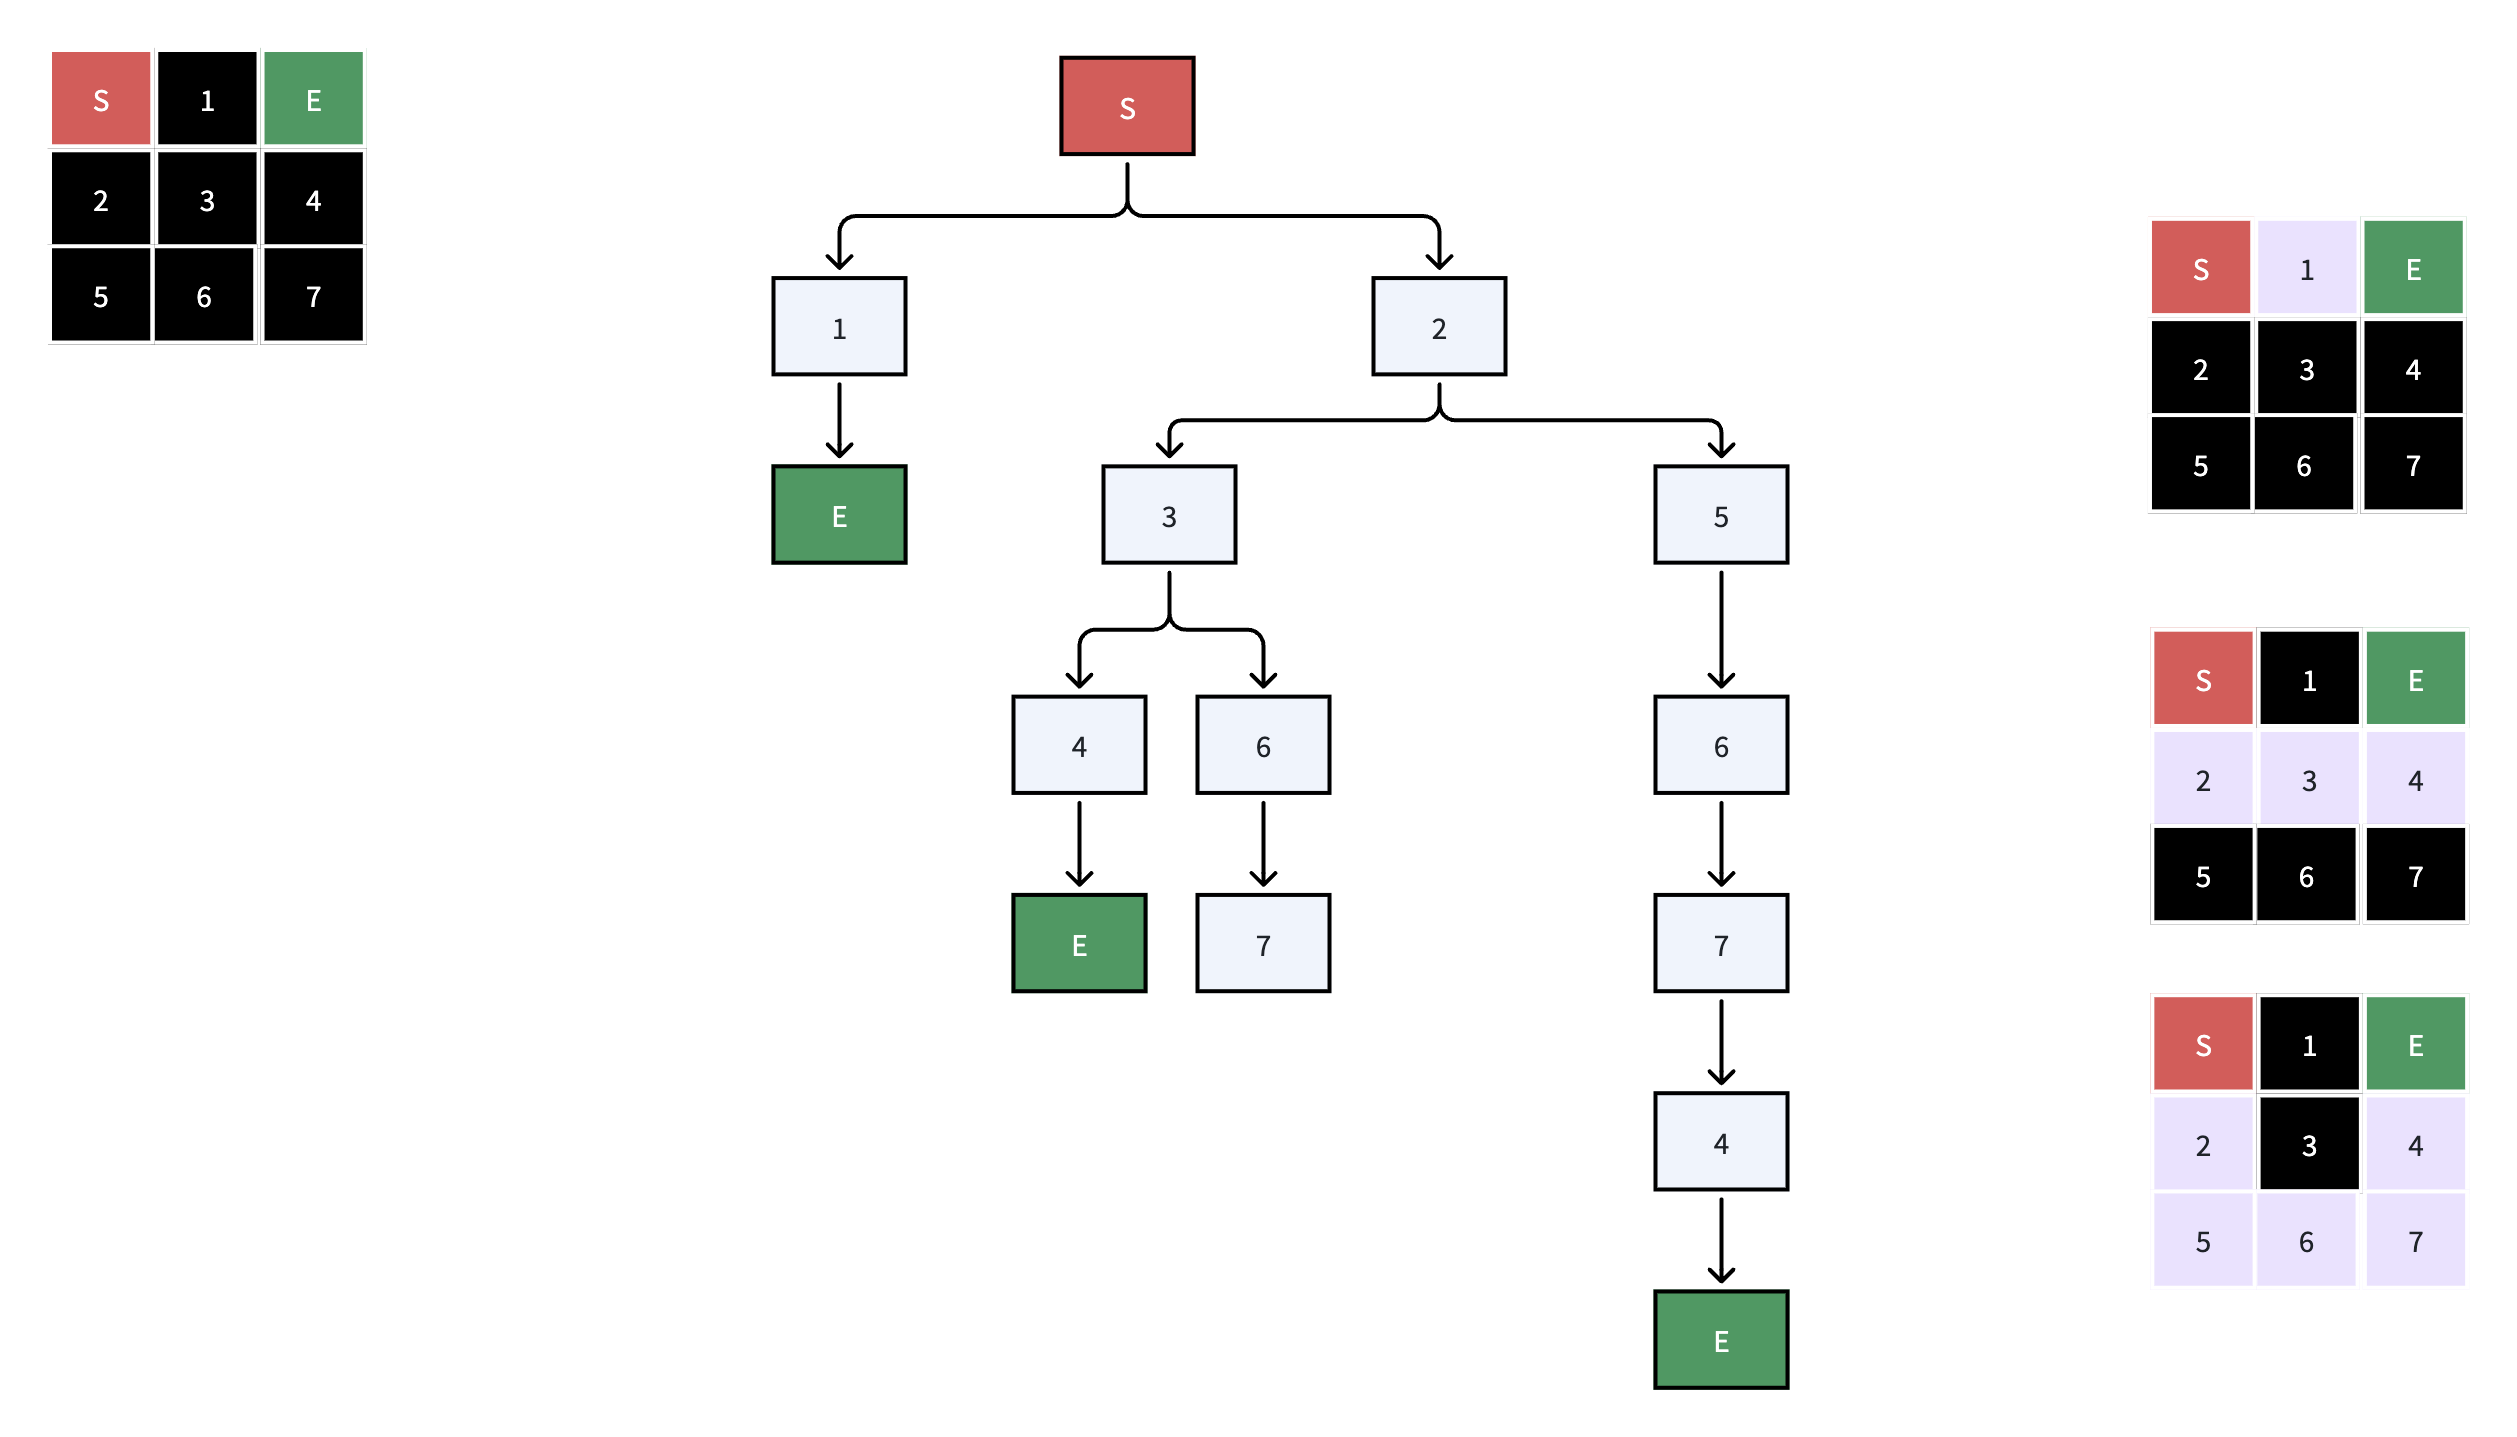
\includegraphics[width=0.95\textwidth]{img/maze-paths-start-0-0-goal-0-2.png}
    \caption{The three valid paths on a $3\times3$ grid with $S=(0,0)$ and $E=(0,2)$. The diagram shows the path search and the resulting traversable cells for each completed path.}
    \label{fig:maze_paths_first_example}
\end{figure}

For a concrete example, in Figure ~\ref{fig:maze_paths_first_example}, consider a $3\times3$ grid with $S=(0,0)$ and $E=(0,2)$. From $S$, we can go to cell 1 and cell 2.

\begin{enumerate}[
    label=\arabic*.,
    leftmargin=*,
    itemsep=1em
]

    \item If we go to cell 1, we can directly go to the goal.
    So for cell 1, there is only one possible path.

    \item Now let's turn to cell 2.
    For cell 2, we can go to the starting point, cell 3, and cell 5.

    \begin{enumerate}[
        label=\alph*.,
        leftmargin=2em,
        itemsep=0.8em
    ]
        \item Here, let's introduce a rule:
        We can't go to a cell that is already on the path
        (the path we are building, not other finished paths,
        like previous $S \to 1 \to E$.
        Here the path means $S \to 2$),
        or to any neighbors of a cell on the path,
        except for the neighbors of the last cell on the path.

        For example, if the path is from $S$ to cell 2
        and we are at cell 2, then we can't go to
        $\{S,2,1\}$, and the neighbors of cell 2 are
        $\{S,3,5\}$, so in this case, the valid neighbors are
        $\{3,5\}$.
    \end{enumerate}
    \item Let's say we go to cell 3.
    Then the valid neighbors of cell 3 are 4 and 6,
    by applying rule 2.a.
    \begin{enumerate}[
        label=\alph*.,
        leftmargin=2em,
        itemsep=0.8em
    ]
        \item For cell 4, it is a neighbor of cell $E$,
        so here we introduce another rule:
        If we are at a cell that is a neighbor of cell $E$,
        the next step can only be to go to cell $E$.

        \item If we choose cell 6 from cell 3,
        and we know the full path is
        \[
            S \to 2 \to 3 \to 6,
        \]
        then the only valid neighbor for cell 6 is 7.
        But for cell 7, there is no valid neighbor,
        so this path ends.
    \end{enumerate}
    \item Let's say we choose cell 5 from cell 2.
    By applying the same two rules, we know the next step
    could only be cell 6, and the next step is cell 7,
    cell 4, and cell $E$.
\end{enumerate}

Figure~\ref{fig:maze_paths_second_example} gives another $3\times3$ example, with $S=(0,0)$ and $E=(2,2)$. The same rules produce six valid paths. For instance, $S\to1\to2\to5\to E$ and $S\to3\to6\to7\to E$ are two different paths.
\begin{figure}[htbp]
    \centering
    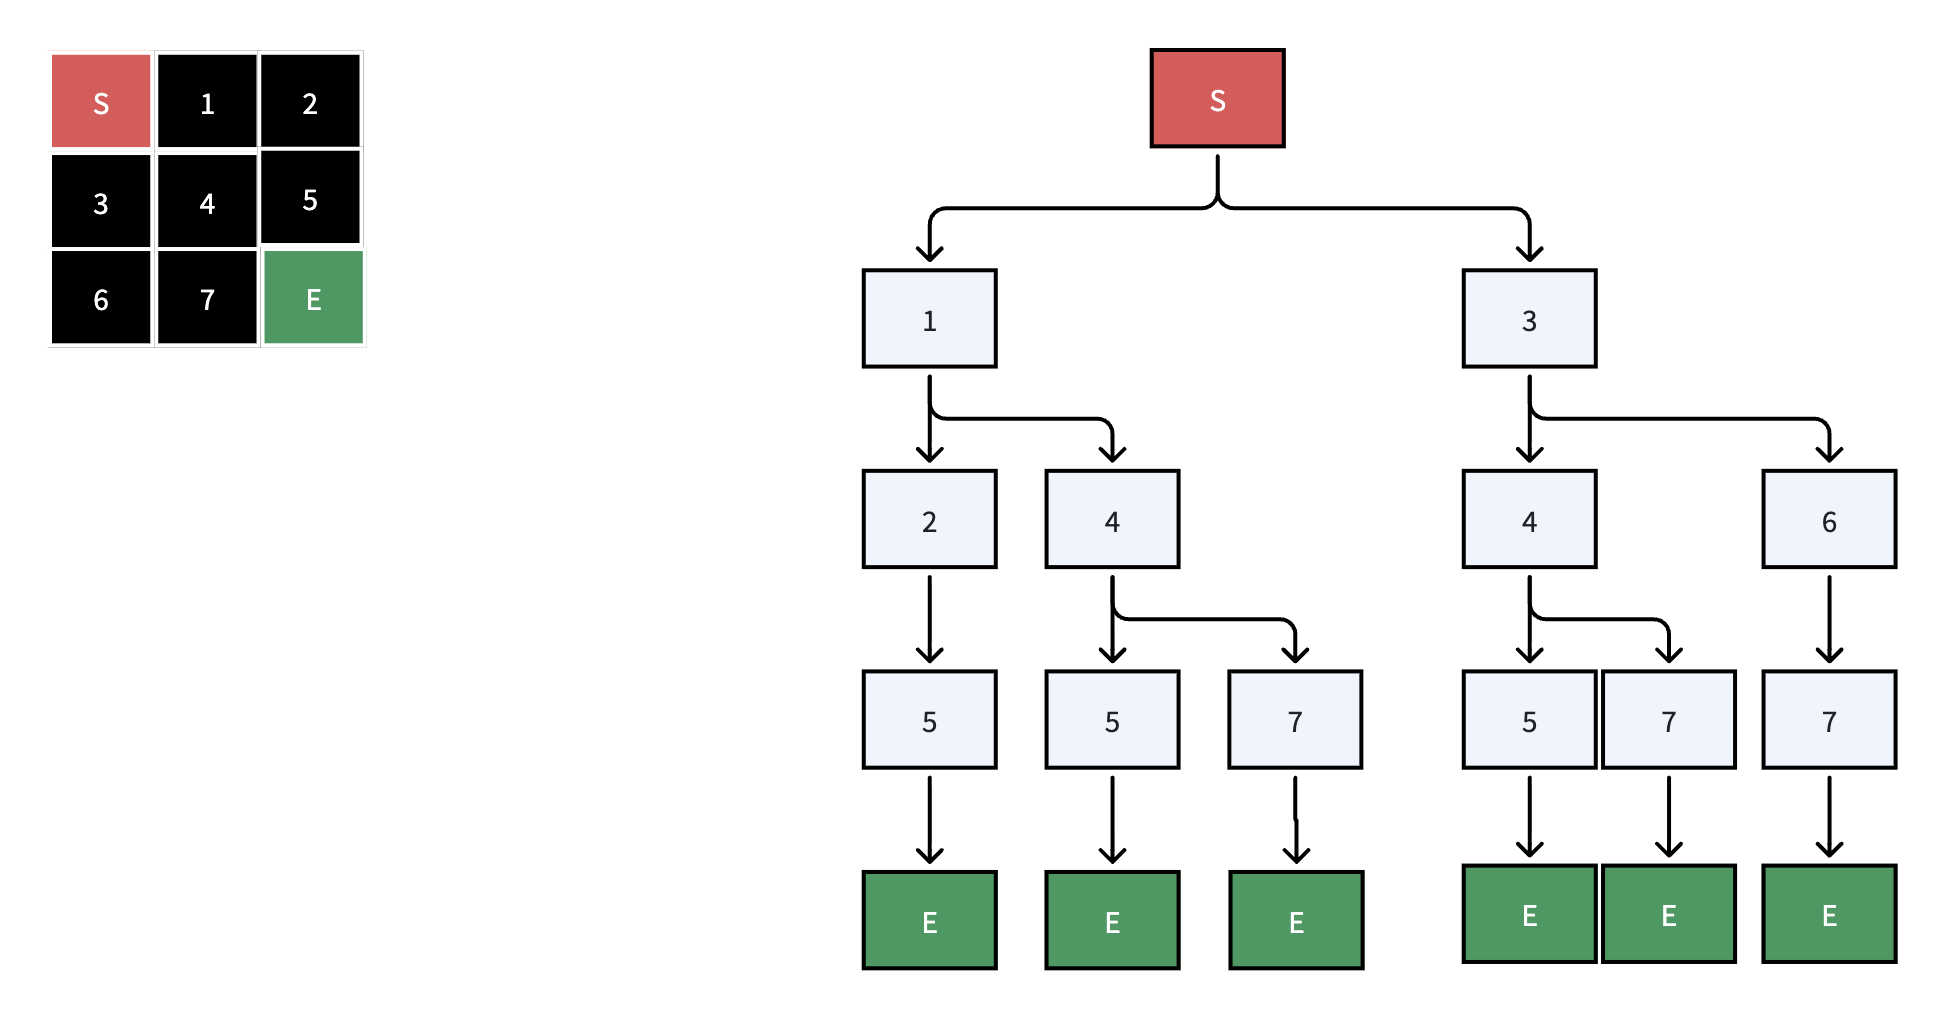
\includegraphics[width=0.95\textwidth]{img/maze-paths-start-0-0-goal-2-2.png}
    \caption{The six valid paths on a $3\times3$ grid with $S=(0,0)$ and $E=(2,2)$.}
    \label{fig:maze_paths_second_example}
\end{figure}


\subsection{Maze variation}

The mazes generated above have only one traversable path from $S$ to $E$; every other cell is an obstacle. These layouts may be too simple for the agent, so we add passages to make the mazes more complex. A single original maze can have many variations. As Figure~\ref{fig:maze_variation_example} illustrates, the maze on the left contains only the original path, while the mazes on the right open different obstacle cells. They retain the same original path as their unique shortest route, although a variation may also contain longer routes.

We first generate the original set using the path-finding algorithm and split it into an original training set and an original test set. We then apply maze variation separately to the two sets. All variations derived from one original maze therefore remain in the same split, so the original solution of a test maze is not introduced into training through its variations.

\paragraph{Variation procedure.}
For each original maze in either split, we perform the following steps:
\begin{enumerate}
    \item Record its original path from $S$ to $E$.
    \item Independently replace each obstacle with a traversable cell with probability $0.5$.
    \item Check the shortest routes from $S$ to $E$. If a shorter route or another equally short route exists, randomly select a traversable cell on such a route that is not part of the original path and turn it back into an obstacle. Repeat this check and repair until the original path is the unique shortest route.
    \item Save the resulting variation and continue with the next original maze.
\end{enumerate}

This procedure creates more complex layouts while preserving the intended optimal solution. The algorithm above is a simple way to create maze variation, which will not ensure we generate all variations of an original maze. In our project, for each original maze, we only generate one maze variation.

\begin{figure}[htbp]
    \centering
    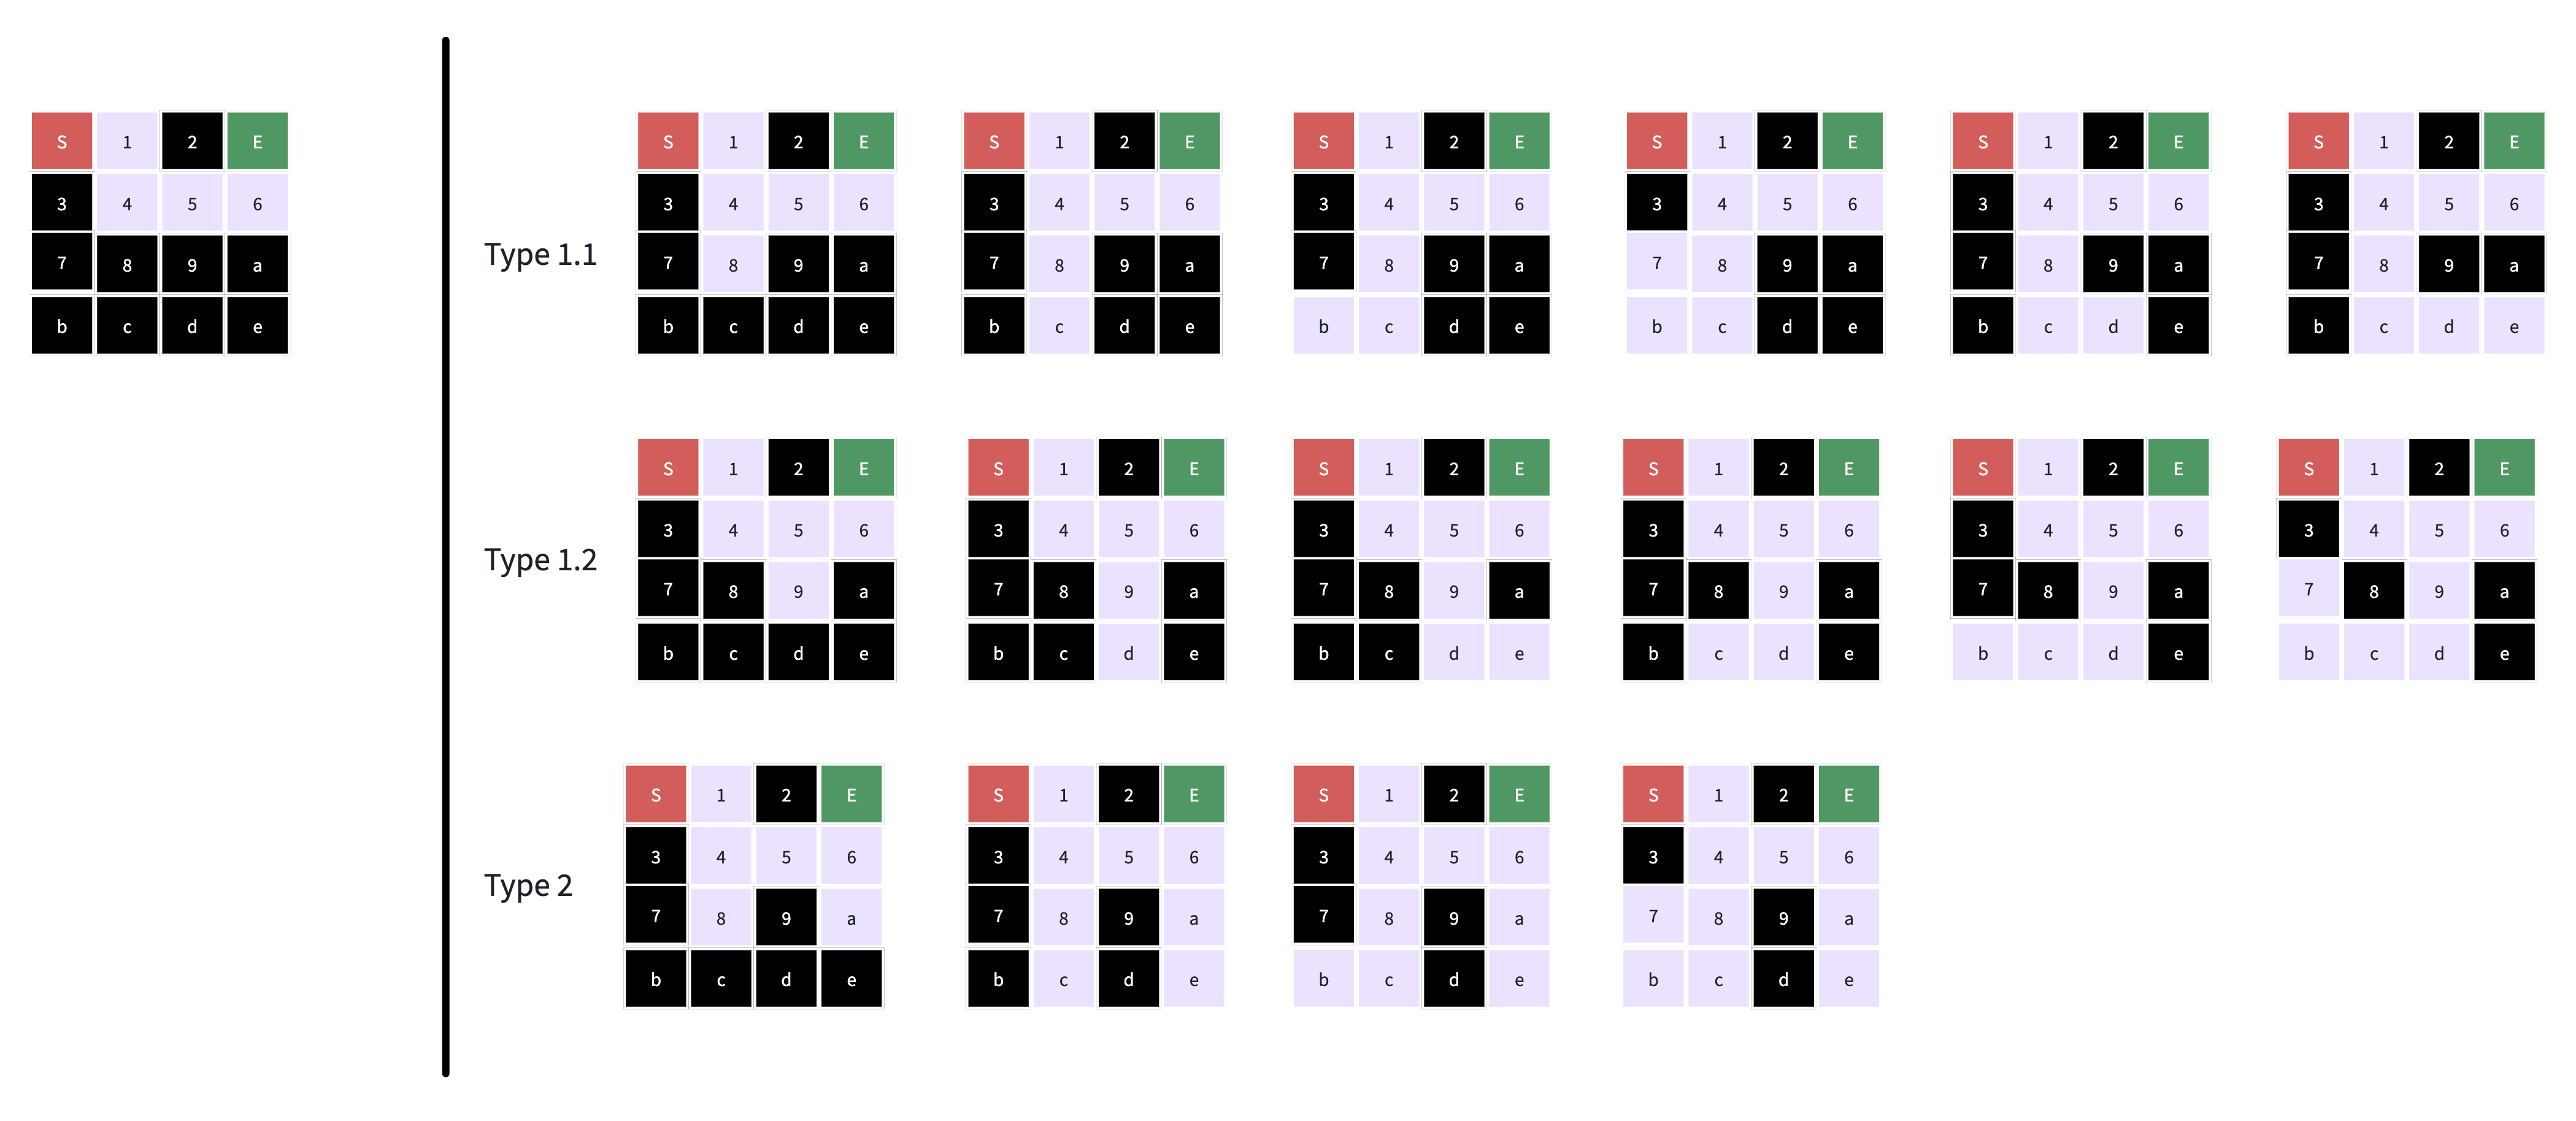
\includegraphics[width=\textwidth]{img/maze-variation-example.png}
    \caption{One original maze (left) and several possible variations (right). Purple cells are traversable, black cells are obstacles, and the variations retain the same optimal route from $S$ to $E$.}
    \label{fig:maze_variation_example}
\end{figure}


\subsection{Observation design}

In designing the observation, we try to make it satisfy the Markov property as much as possible. In other words, the information the agent needs to make a decision should be contained in its current observation. This reduces interference from partial observability.

The observation has three parts:
\begin{enumerate}
    \item \textbf{Representation of reachable path cells and obstacles.} We use $1$ for a reachable, walkable cell and $0$ for an obstacle.
    \item \textbf{The agent's row and column.} Two column vectors represent the row and column in which the agent is located, respectively.
    \item \textbf{The goal's location.} Similarly, two column vectors represent the goal's row and column, respectively.
\end{enumerate}

Figure~\ref{fig:maze_observation_design} shows how these three parts are placed together in a two-dimensional observation array. The four position columns use one-hot encoding for the agent's row and column and the goal's row and column.

\begin{figure}[htbp]
    \centering
    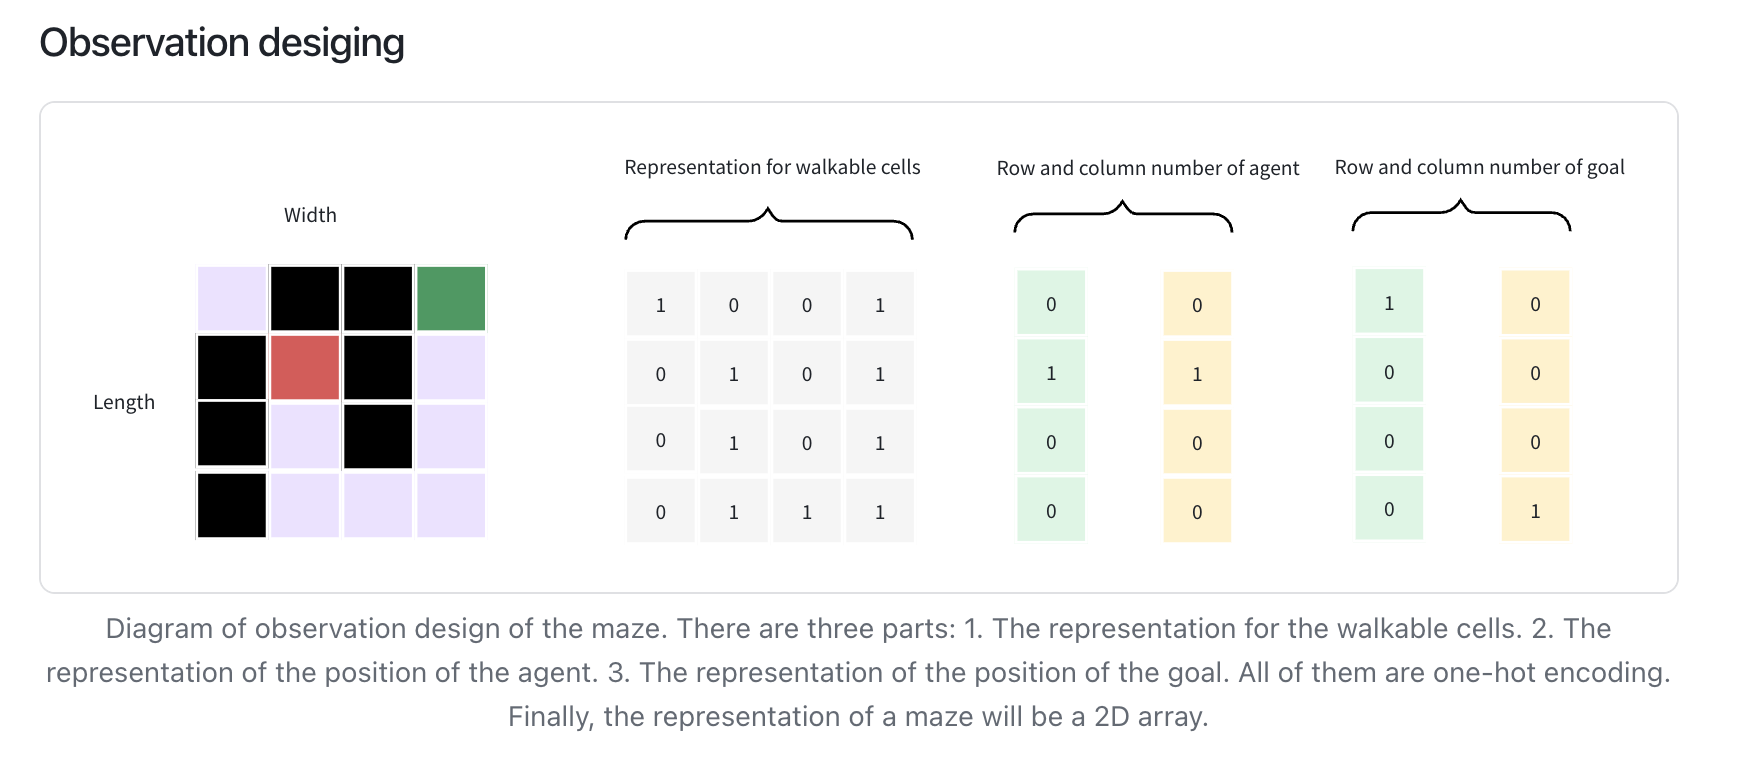
\includegraphics[width=\textwidth]{img/maze-observation-design.png}
    \caption{Observation design for a maze: a binary map of walkable cells and obstacles, followed by separate one-hot column vectors for the agent's and goal's row and column. There are three parts: 1. The representation for the walkable cells. 2. The representation of the position of the agent. 3. The representation of the position of the goal. All of them are one-hot encoding. Finally, the representation of a maze will be a 2D array.}
    \label{fig:maze_observation_design}
\end{figure}

\section{Actor DQN}

This section describes the intended model design. Actor DQN keeps the online Q network and target Q network of a normal DQN, and adds a separate actor Q network. The actor Q network produces one score for each action. A softmax layer converts these scores into an action-probability distribution, as illustrated in Figure~\ref{fig:actor_dqn_design}.

In this design, the training label for a state $s$ is the action with the highest value according to the DQN online network:
\begin{equation}
    y(s) = \arg\max_a Q_{\mathrm{online}}(s,a).
\end{equation}
The actor Q network is trained against this label using cross-entropy loss. If $z_{\mathrm{actor}}(s,a)$ is its score for action $a$, its policy and loss are
\begin{equation}
    \pi_{\mathrm{actor}}(a\mid s)
    = \frac{\exp(z_{\mathrm{actor}}(s,a))}
           {\sum_{a'}\exp(z_{\mathrm{actor}}(s,a'))},
    \qquad
    \mathcal{L}_{\mathrm{actor}}(s)
    = -\log\pi_{\mathrm{actor}}(y(s)\mid s).
\end{equation}

Training rollouts follow the normal DQN rollout procedure: actions are selected using the online DQN Q network with its exploration strategy. The actor Q network does not select actions during these rollouts. It is used for evaluation, where an action is sampled from its softmax probability distribution.

\begin{figure}[H]
    \centering
    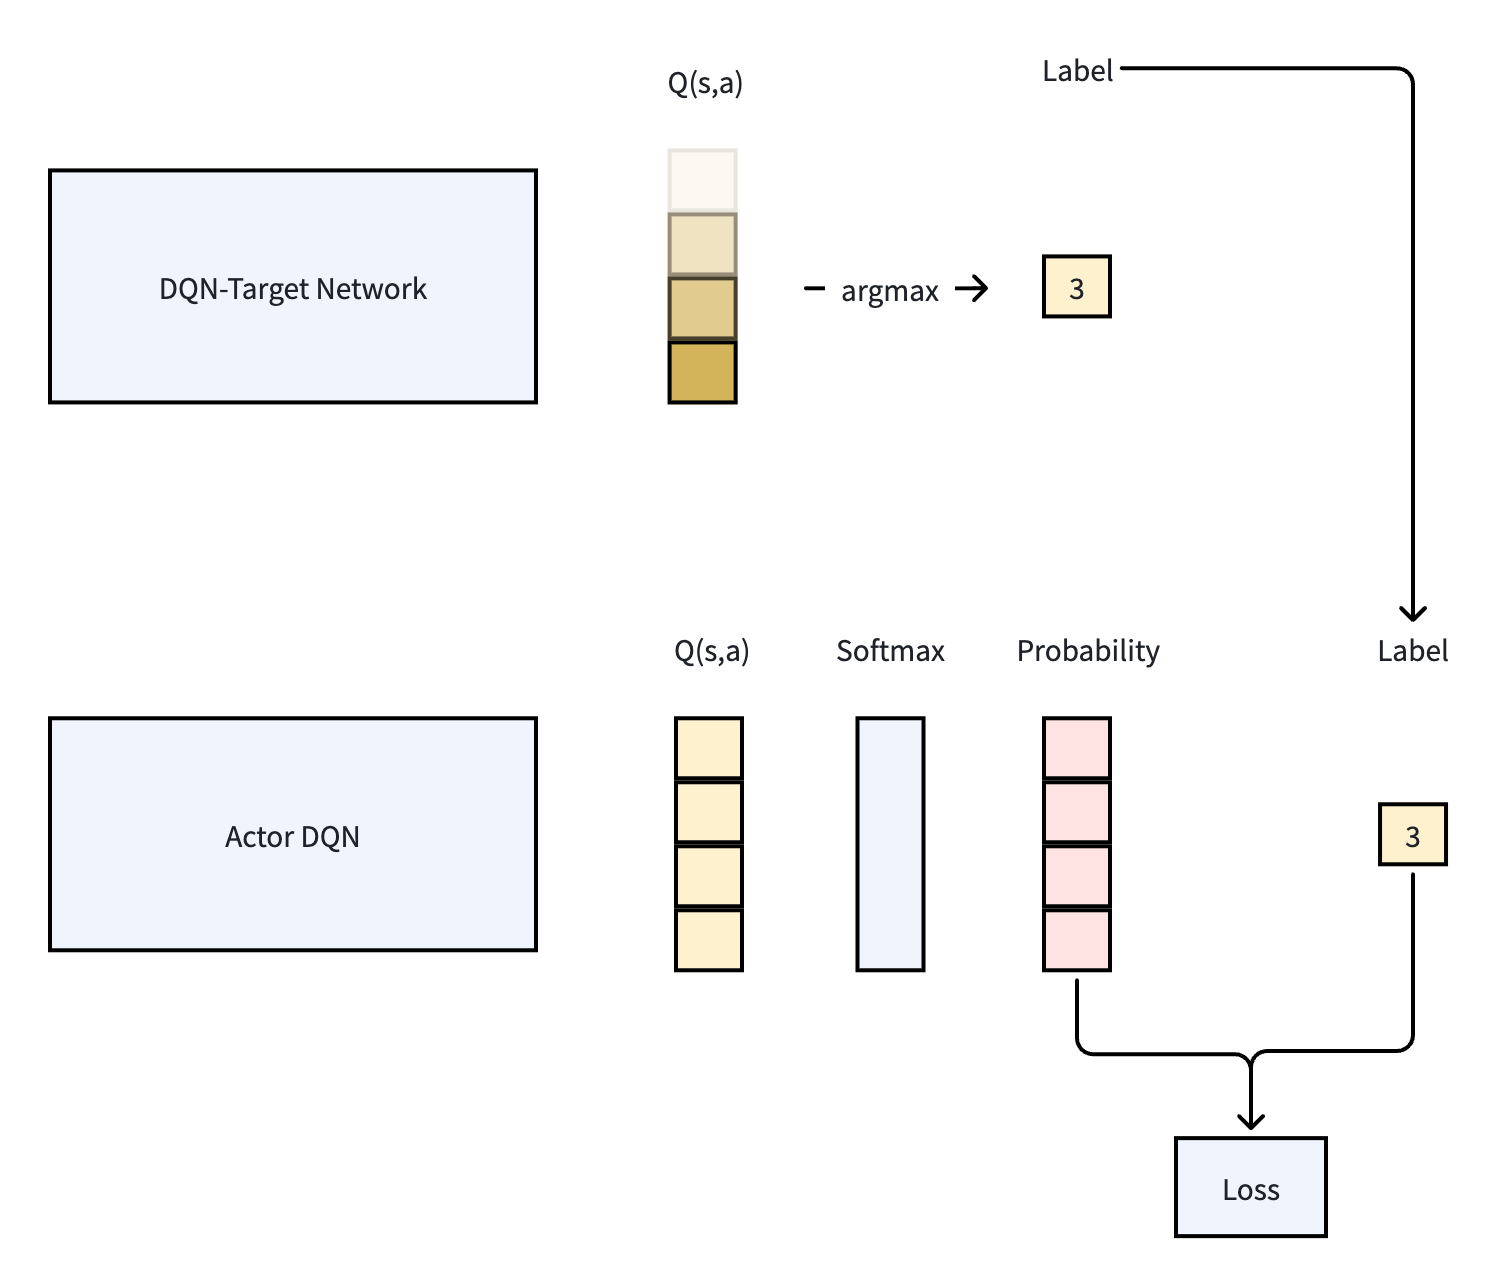
\includegraphics[width=0.88\textwidth]{img/actor-dqn-design.png}
    \caption{Actor DQN design. The DQN online network provides an action label through an argmax operation, while the additional actor Q network produces action scores that are converted into probabilities by softmax.}
    \label{fig:actor_dqn_design}
\end{figure}


\FloatBarrier
\section{Experiment}

In the maze task, the agent starts at a designated cell and must reach the goal cell by moving up, down, left, or right. We compare four policies on the validation mazes:
\begin{enumerate}
    \item \textbf{Actor DQN} has three Q networks: an online network, a target network, and an actor network. At evaluation time, actions are sampled from the actor network's softmax distribution.
    \item \textbf{Basic DQN} has an online Q network and a target Q network. Its training rollouts use a fixed $\varepsilon$-greedy strategy with $\varepsilon=0.1$: 90\% exploitation and 10\% exploration. The results in the tables below use greedy action selection from the saved online network during evaluation. For Actor DQN, it also uses the same training rollouts as Basic DQN.
    \item \textbf{Random Actor} uses the randomly initialized actor network of an ActorDQN whose network parameters were not trained. Evaluation actions are sampled from this actor's softmax distribution.
    \item \textbf{Uniform Random} selects each of the four actions with probability 25\% at every state.
\end{enumerate}


All Q networks use a multilayer perceptron (MLP) with hidden-layer widths of 128, 128, 64, and 32. Each hidden layer consists of a linear layer, followed by Layer Normalization and a ReLU activation. A final linear layer produces one Q value for each of the four actions.

The maximum number of steps per episode is the same for training and validation. We set it to ten times the number of cells in the maze: $4\times4\times10=160$ steps for a $4\times4$ maze, and $5\times5\times10=250$ steps for a $5\times5$ maze.


The tables report three metrics on the full validation set. \emph{Mean Steps (All)} is the total number of steps across all mazes divided by the number of mazes, including both successful and truncated episodes. \emph{Mean Steps (Success)} is the average number of steps among episodes that reach the goal. \emph{Success Rate} is the number of mazes solved divided by the total number of validation mazes. Each table entry is the mean across three seeds, followed by the sample standard deviation.

\begin{table}[htbp]
    \centering
    \caption{Performance on Maze4x4}
    \begin{tabular}{lccc}
        \hline
        Policy 
        & Mean Steps (All)
        & Mean Steps (Success)
        & Success Rate \\
        \hline

        ActorDQN
        & $\mathbf{49.01 \pm 6.60}$
        & $25.95 \pm 3.65$
        & $\mathbf{0.828 \pm 0.029}$ \\

        Basic DQN
        & $142.76 \pm 11.22$
        & $\mathbf{4.42 \pm 0.94}$
        & $0.111 \pm 0.072$ \\

        Random Actor
        & $103.08 \pm 28.63$
        & $60.71 \pm 5.67$
        & $0.566 \pm 0.265$ \\

        Uniform Random
        & $88.87 \pm 5.74$
        & $63.86 \pm 4.04$
        & $0.740 \pm 0.048$ \\

        \hline
    \end{tabular}
    \label{tab:maze4x4}
\end{table}

\begin{table}[htbp]
    \centering
    \caption{Performance on Maze5x5}
    \begin{tabular}{lccc}
        \hline
        Policy 
        & Mean Steps (All)
        & Mean Steps (Success)
        & Success Rate \\
        \hline

        ActorDQN
        & $\mathbf{114.11 \pm 8.80}$
        & $48.26 \pm 5.09$
        & $\mathbf{0.673 \pm 0.027}$ \\

        Basic DQN
        & $218.71 \pm 8.52$
        & $\mathbf{8.33 \pm 0.45}$
        & $0.129 \pm 0.036$ \\

        Random Actor
        & $189.21 \pm 15.92$
        & $119.45 \pm 3.69$
        & $0.464 \pm 0.109$ \\

        Uniform Random
        & $178.01 \pm 0.43$
        & $122.25 \pm 1.22$
        & $0.564 \pm 0.004$ \\

        \hline
    \end{tabular}
    \label{tab:maze5x5}
\end{table}

\FloatBarrier
\subsection{Results and Analysis}

Table~\ref{tab:maze4x4} shows that ActorDQN takes the fewest steps when averaged over all 4$\times$4 validation mazes (49.01) and achieves the highest success rate (0.828). Basic DQN takes the fewest steps among the mazes it solves (4.42), but its success rate is only 0.111. One possible explanation is that it succeeds mainly on easy mazes, such as those where the goal is only one or two moves from the start. In that case, its successful episodes would be short even though it fails on most mazes.

The 5$\times$5 results in Table~\ref{tab:maze5x5} show the same overall pattern. ActorDQN again has the fewest steps across all validation mazes (114.11) and the highest success rate (0.673). Among successful episodes, it also takes fewer steps (48.26) than Random Actor (119.45) and Uniform Random (122.25). Basic DQN has a still lower success-only mean (8.33), but reaches the goal in only 0.129 of the validation mazes.

\subsection{Training Performance and Generalization Gap}

Tables~\ref{tab:train_maze4x4} and~\ref{tab:train_maze5x5} report performance on the full training sets using the same checkpoints and evaluation procedure as above. Each seed has 803 training mazes for the 4$\times$4 environment and 11,891 for the 5$\times$5 environment. As in the validation tables, entries show the mean and sample standard deviation across three seeds.

\begin{table}[htbp]
    \centering
    \caption{Training-set performance on 4$\times$4 mazes.}
    \begin{tabular}{lccc}
        \hline
        Policy & Mean Steps (All) & Mean Steps (Success) & Success Rate \\
        \hline
        ActorDQN & $\mathbf{42.94 \pm 11.52}$ & $23.03 \pm 4.25$ & $\mathbf{0.853 \pm 0.058}$ \\
        Basic DQN & $127.04 \pm 25.23$ & $\mathbf{4.53 \pm 1.37}$ & $0.213 \pm 0.163$ \\
        Random Actor & $99.75 \pm 30.62$ & $59.56 \pm 5.84$ & $0.590 \pm 0.278$ \\
        Uniform Random & $85.74 \pm 3.71$ & $61.96 \pm 2.15$ & $0.757 \pm 0.024$ \\
        \hline
    \end{tabular}
    \label{tab:train_maze4x4}
\end{table}

\begin{table}[htbp]
    \centering
    \caption{Training-set performance on 5$\times$5 mazes.}
    \begin{tabular}{lccc}
        \hline
        Policy & Mean Steps (All) & Mean Steps (Success) & Success Rate \\
        \hline
        ActorDQN & $\mathbf{110.21 \pm 13.01}$ & $46.94 \pm 5.52$ & $\mathbf{0.688 \pm 0.046}$ \\
        Basic DQN & $216.88 \pm 9.78$ & $\mathbf{8.36 \pm 0.34}$ & $0.137 \pm 0.041$ \\
        Random Actor & $189.19 \pm 14.25$ & $118.87 \pm 3.78$ & $0.462 \pm 0.099$ \\
        Uniform Random & $177.23 \pm 0.97$ & $123.44 \pm 0.33$ & $0.575 \pm 0.007$ \\
        \hline
    \end{tabular}
    \label{tab:train_maze5x5}
\end{table}

For each metric, we define the generalization gap as the three-seed training mean minus the three-seed validation mean. A positive success-rate gap indicates higher success on training mazes; a negative Mean Steps (All) gap indicates fewer steps on training mazes. Therefore, the smaller the absolute value of the gap, the better the generalisation performance. Table~\ref{tab:generalization_gap} reports differences between means.

\begin{table}[htbp]
    \centering
    \small
    \caption{Generalization gaps: training-set mean minus validation-set mean. For each metric, a smaller absolute gap is better.}
    \begin{tabular}{llrrr}
        \hline
        Maze & Policy & \shortstack{$\Delta$ Steps (All)\\$|\Delta|\downarrow$} & \shortstack{$\Delta$ Steps (Success)\\$|\Delta|\downarrow$} & \shortstack{$\Delta$ Success Rate\\$|\Delta|\downarrow$} \\
        \hline
        4$\times$4 & ActorDQN & $\mathbf{-6.07}$ & $-2.92$ & $\mathbf{+0.026}$ \\
        & Basic DQN & $-15.72$ & $\mathbf{+0.12}$ & $+0.102$ \\
        \hline
        5$\times$5 & ActorDQN & $-3.89$ & $-1.32$ & $+0.014$ \\
        & Basic DQN & $\mathbf{-1.83}$ & $\mathbf{+0.03}$ & $\mathbf{+0.008}$ \\
        \hline
    \end{tabular}
    \label{tab:generalization_gap}
\end{table}

\FloatBarrier
For 4$\times$4 mazes, ActorDQN has a smaller gap than Basic DQN in both success rate (0.026 versus 0.102) and the absolute value of Mean Steps (All) (6.07 versus 15.72). This is consistent with the expected ordering for 4$\times$4 mazes. The 5$\times$5 results do not follow the same ordering: Basic DQN has a smaller success-rate gap (0.008 versus 0.014) and a smaller absolute Mean Steps (All) gap (1.83 versus 3.89). However, its validation success rate is only 0.129, compared with 0.673 for ActorDQN. A small gap can therefore coexist with poor performance on both splits; it does not by itself show that Basic DQN solves unseen mazes better.

\subsection{Classification and Q-Value Regression Probe}

To examine the proposed classification mechanism more directly, we use two frozen teacher networks from the 4$\times$4 maze experiments: the DQN target Q network and the ActorDQN target Q network. Each teacher is used to generate both kinds of label for the same observation $s$:
\begin{equation}
    y_{\mathrm{reg}}(s)=\bigl(Q_{\mathrm{target}}(s,a)\bigr)_{a=1}^{4},
    \qquad
    y_{\mathrm{cls}}(s)=\arg\max_a Q_{\mathrm{target}}(s,a).
\end{equation}
For each teacher, one student Q network fits the four Q values using mean squared error; another student with the same architecture predicts the best action using cross-entropy. This gives four teacher--objective combinations. The students start from identical weights and receive identical minibatches within a run. The teacher parameters remain frozen.

We collect 102,400 state transitions with a uniformly random policy to sample transitions on the 4$\times$4 training mazes. Each student receives 102,400 minibatch updates with batch size 64 and learning rate $10^{-3}$. At evaluation time, both objectives select the highest-scoring action with $\arg\max$; this keeps the action-selection rule fixed while the training label changes. We measure agreement with the frozen teacher's greedy action on the held-out observations, and separately measure the fraction of unseen validation mazes solved within 160 actions. 

\paragraph{Action agreement}
For each held-out observation $s_i$, we compare the student's greedy action with the action preferred by its frozen teacher:
\begin{equation}
    \mathrm{Action\ Agreement}
    = \frac{1}{N}\sum_{i=1}^{N}
    \mathbf{1}\!\left[
        \arg\max_a z_{\theta}(s_i,a)
        =
        \arg\max_a Q_{\mathrm{target}}(s_i,a)
    \right].
\end{equation}
Here $z_{\theta}$ denotes the student's output: action logits for classification and predicted Q values for regression. Thus, action agreement is the fraction of held-out observations on which the student chooses the same action as its teacher. It measures how well the student reproduces the teacher's decision, not whether that action is optimal or whether the student completes a maze.

\begin{table}[htbp]
    \centering
    \small
    \caption{Classification and regression students trained from frozen target-network labels on 4$\times$4 mazes (seed 42). Action agreement is measured against each teacher's greedy action on held-out observations. Maze success is measured after 102,400 updates on the 201 unseen validation mazes.}
    \begin{tabular}{llccc}
        \hline
        Teacher & Student objective & \shortstack{Action agreement\\10,000 updates} & \shortstack{Action agreement\\102,400 updates} & \shortstack{Maze success\\102,400 updates} \\
        \hline
        DQN & Classification & $\mathbf{0.868}$ & $\mathbf{0.899}$ & $\mathbf{137/201\;(0.682)}$ \\
            & Q-value regression & $0.800$ & $0.853$ & $116/201\;(0.577)$ \\
        \hline
        ActorDQN & Classification & $\mathbf{0.964}$ & $\mathbf{0.967}$ & $\mathbf{175/201\;(0.871)}$ \\
                 & Q-value regression & $0.910$ & $0.955$ & $162/201\;(0.806)$ \\
        \hline
    \end{tabular}
    \label{tab:classification_regression_probe}
\end{table}

For both frozen teachers, classification has higher held-out action agreement after 10,000 updates and at the final update. It also solves more validation mazes: 137 versus 116 for the DQN teacher, and 175 versus 162 for the ActorDQN teacher. Thus, with the same network architecture, initial weights, observations, update budget, and greedy evaluation rule, learning the teacher's preferred action performs better here than fitting all four numerical Q values. This supports the classification hypothesis for this probe. The result is from one seed and uses the teacher's preferred action as the state-level reference, rather than an independently known optimal action. It does not, by itself, establish that this mechanism explains the performance difference between the complete ActorDQN and DQN agents.

\section{Conclusion}

This study evaluated whether an auxiliary actor trained to predict a Q network's preferred action can improve maze navigation on unseen layouts. Across three seeds, ActorDQN achieved higher validation success than Basic DQN on both maze sizes: $0.828$ versus $0.111$ on 4$\times$4 mazes, and $0.673$ versus $0.129$ on 5$\times$5 mazes. Its validation episodes also required fewer steps on average. The training--validation success gap was smaller for ActorDQN on 4$\times$4 mazes, but not on 5$\times$5 mazes; the gap alone therefore does not establish which policy generalizes better.

The separate frozen-teacher probe provides evidence for one possible mechanism. With identical student architectures, initial weights, minibatches, and greedy evaluation, classification students matched their teachers' preferred actions more often and solved more unseen 4$\times$4 mazes than students trained to regress all four Q values. This supports the idea that learning an action decision can be easier than fitting precise Q values in this setting. 


\clearpage
\begin{thebibliography}{9}

\bibitem{wang2026}
Guo Bohao.
\newblock Wang Xingxing: The ``ChatGPT moment'' for embodied intelligence could arrive in two to three years; physical AI self-evolution could enable robots at scale.
\newblock People's Financial News, August 20, 2026. In Chinese.
\newblock \url{https://www.stcn.com/article/detail/4090340.html}.

\bibitem{cobbe2020}
Karl Cobbe, Chris Hesse, Jacob Hilton, and John Schulman.
\newblock Leveraging Procedural Generation to Benchmark Reinforcement Learning.
\newblock In \emph{Proceedings of the 37th International Conference on Machine Learning}, pages 2048--2056, 2020.
\newblock \url{https://proceedings.mlr.press/v119/cobbe20a.html}.

\bibitem{openai2019}
OpenAI.
\newblock Procgen Benchmark.
\newblock 2019.
\newblock \url{https://openai.com/index/procgen-benchmark/}.

\bibitem{procgenrepo}
OpenAI.
\newblock Procgen Benchmark environment repository.
\newblock \url{https://github.com/openai/procgen}.

\end{thebibliography}

\end{document}
